\documentclass[12pt, a4paper]{article}  

\usepackage{etex} % расширение классического tex в частности позволяет подгружать гораздо больше пакетов, чем мы и займёмся далее

%%%%%%%%%% Математика %%%%%%%%%%
\usepackage{amsmath,amsfonts,amssymb,amsthm,mathtools} 
%\mathtoolsset{showonlyrefs=true}  % Показывать номера только у тех формул, на которые есть \eqref{} в тексте.
%\usepackage{leqno} % Нумерация формул слева


%%%%%%%%%%%%%%%%%%%%%%%% Шрифты %%%%%%%%%%%%%%%%%%%%%%%%%%%%%%%%%
\usepackage{fontspec}         % пакет для подгрузки шрифтов
\setmainfont{Roboto}   % задаёт основной шрифт документа

% why do we need \newfontfamily:
% http://tex.stackexchange.com/questions/91507/
\newfontfamily{\cyrillicfonttt}{Roboto}
\newfontfamily{\cyrillicfont}{Roboto}
\newfontfamily{\cyrillicfontsf}{Roboto}
% Иногда тех не видит структуры шрифтов. Эти трое бравых парней спасают ситуацию и доопределяют те куски, которые Тех не увидел.

\usepackage{unicode-math}     % пакет для установки математического шрифта
\setmathfont{Asana Math}      % шрифт для математики

\usepackage{polyglossia}      % Пакет, который позволяет подгружать русские буквы
\setdefaultlanguage{russian}  % Основной язык документа
\setotherlanguage{english}    % Второстепенный язык документа



%%%%%%%%%% Работа с картинками %%%%%%%%%
\usepackage{graphicx}                  % Для вставки рисунков
\usepackage{graphics} 
\graphicspath{{images/}{pictures/}}    % можно указать папки с картинками
\usepackage{wrapfig}                   % Обтекание рисунков и таблиц текстом
\usepackage{subfigure}                 % для создания нескольких рисунков внутри одного


%%%%%%%%%% Работа с таблицами %%%%%%%%%%
\usepackage{tabularx}            % новые типы колонок
\usepackage{tabulary}            % и ещё новые типы колонок
\usepackage{array}               % Дополнительная работа с таблицами
\usepackage{longtable}           % Длинные таблицы
\usepackage{multirow}            % Слияние строк в таблице
\usepackage{float}               % возможность позиционировать объекты в нужном месте 
\usepackage{booktabs}            % таблицы как в книгах!  
\renewcommand{\arraystretch}{1.3} % больше расстояние между строками

\begin{document} 

\begin{figure}[H]
\begin{minipage}[h]{0.3\linewidth}
\center{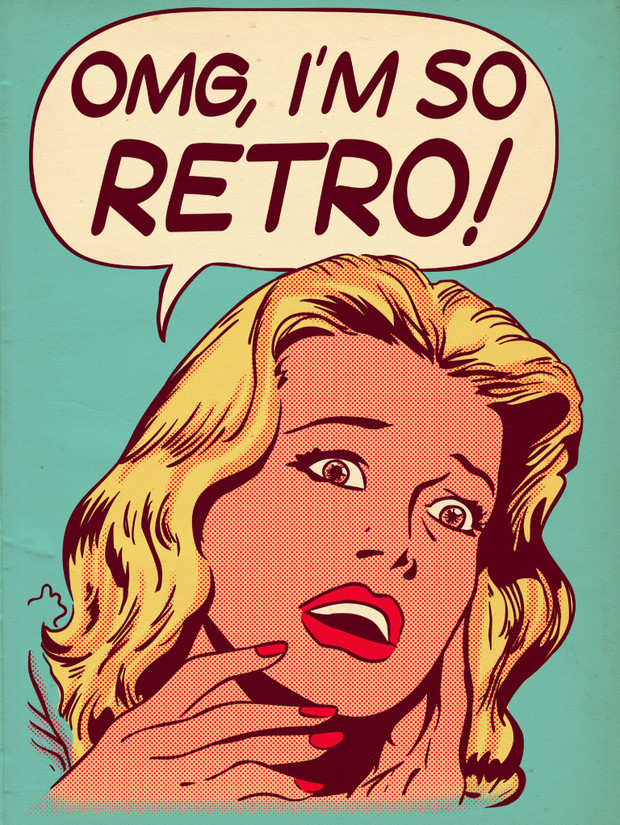
\includegraphics[width=1\linewidth]{pop1.jpg}}
\end{minipage}
\hfill
\begin{minipage}[h]{0.3\linewidth}
\center{
\includegraphics[width=1\linewidth]{pop2.jpg}}
\end{minipage}
\hfill
\begin{minipage}[h]{0.3\linewidth}
\center{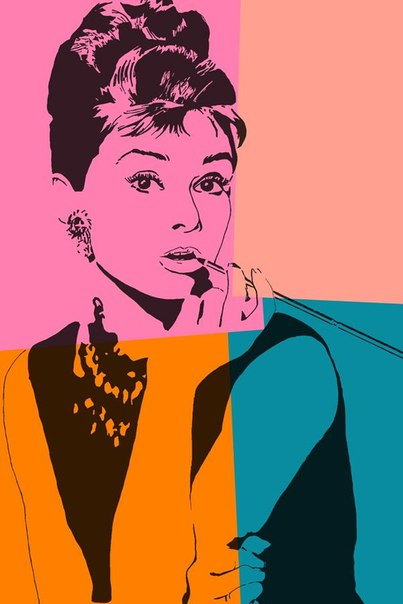
\includegraphics[width=1\linewidth]{pop3.jpg}}
\end{minipage}
\vfill
\begin{minipage}[h]{0.3\linewidth}
\center{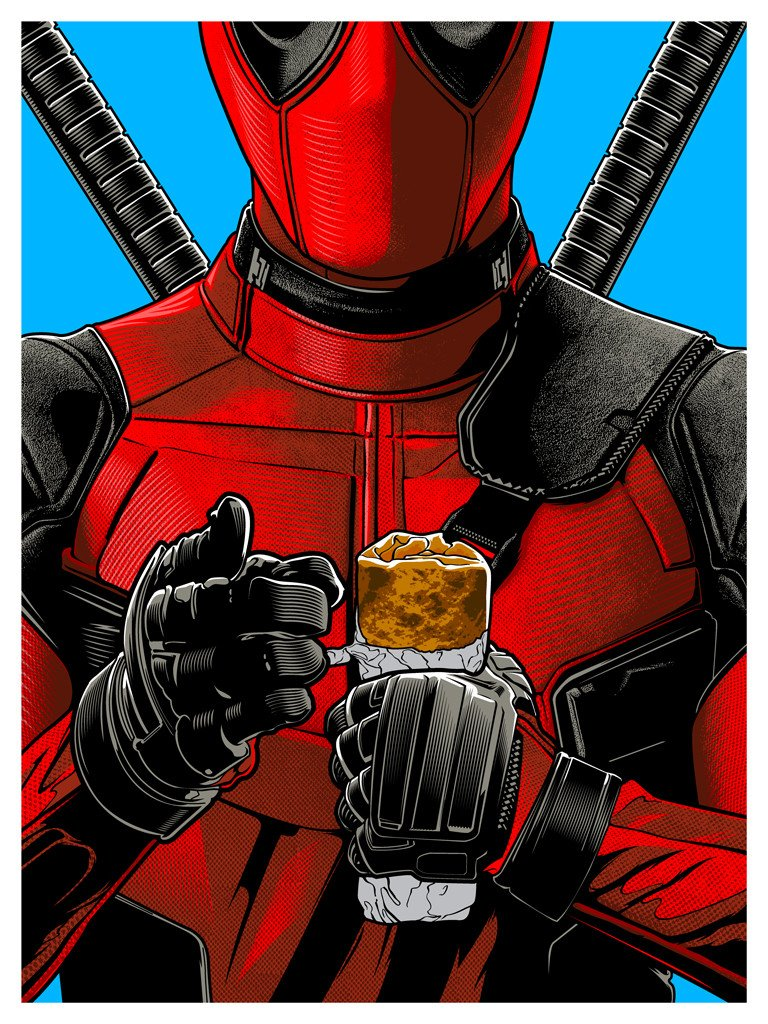
\includegraphics[width=1\linewidth]{pop4.jpg}}
\end{minipage}
\hfill
\begin{minipage}[h]{0.3\linewidth}
\center{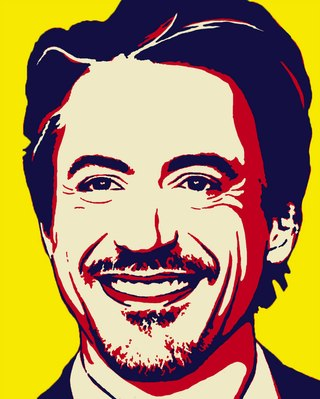
\includegraphics[width=1\linewidth]{pop5.jpg}}
\end{minipage}
\hfill
\begin{minipage}[h]{0.3\linewidth}
\center{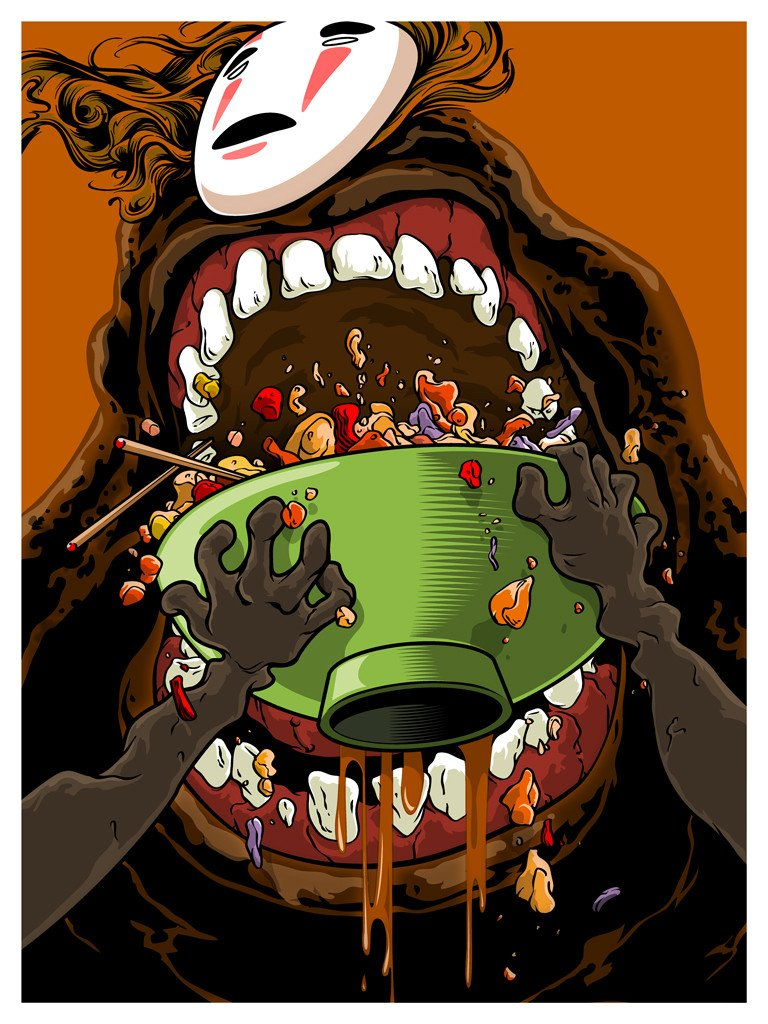
\includegraphics[width=1\linewidth]{pop6.jpg}}
\end{minipage}
\caption{Это что, поп арт?}

\end{figure}


\end{document}